\section{BlaBlaCar}
\label{analyza:blablacar}

BlaBlaCar je přední světová komunita spolujízdy, která spojuje řidiče a cestující na stejné trase, a umožňuje tak levné meziměstské cestování \cite{blablacar}.

Na základě tohoto jednoduchého principu si lidé mohou přisednout k~někomu jako spolucestující. Tímto způsobem se tak dostanou k~častokrát levnější a pohodlnější formě přepravy. Pro řidiče je výhodou částečné proplacení jízdy (pohonných hmot) těmito spolucestujícími.

Níže jsou uvedeny všechny důležité stránky webu BlaBlaCar a u~každé takové stránky je definován seznam pozitivních a negativních vlastností.

\subsection{Hlavní stránka}
Viz obrázek \ref{fig:blablacar:homepage}.
\begin{figure}[h]
    \centering
    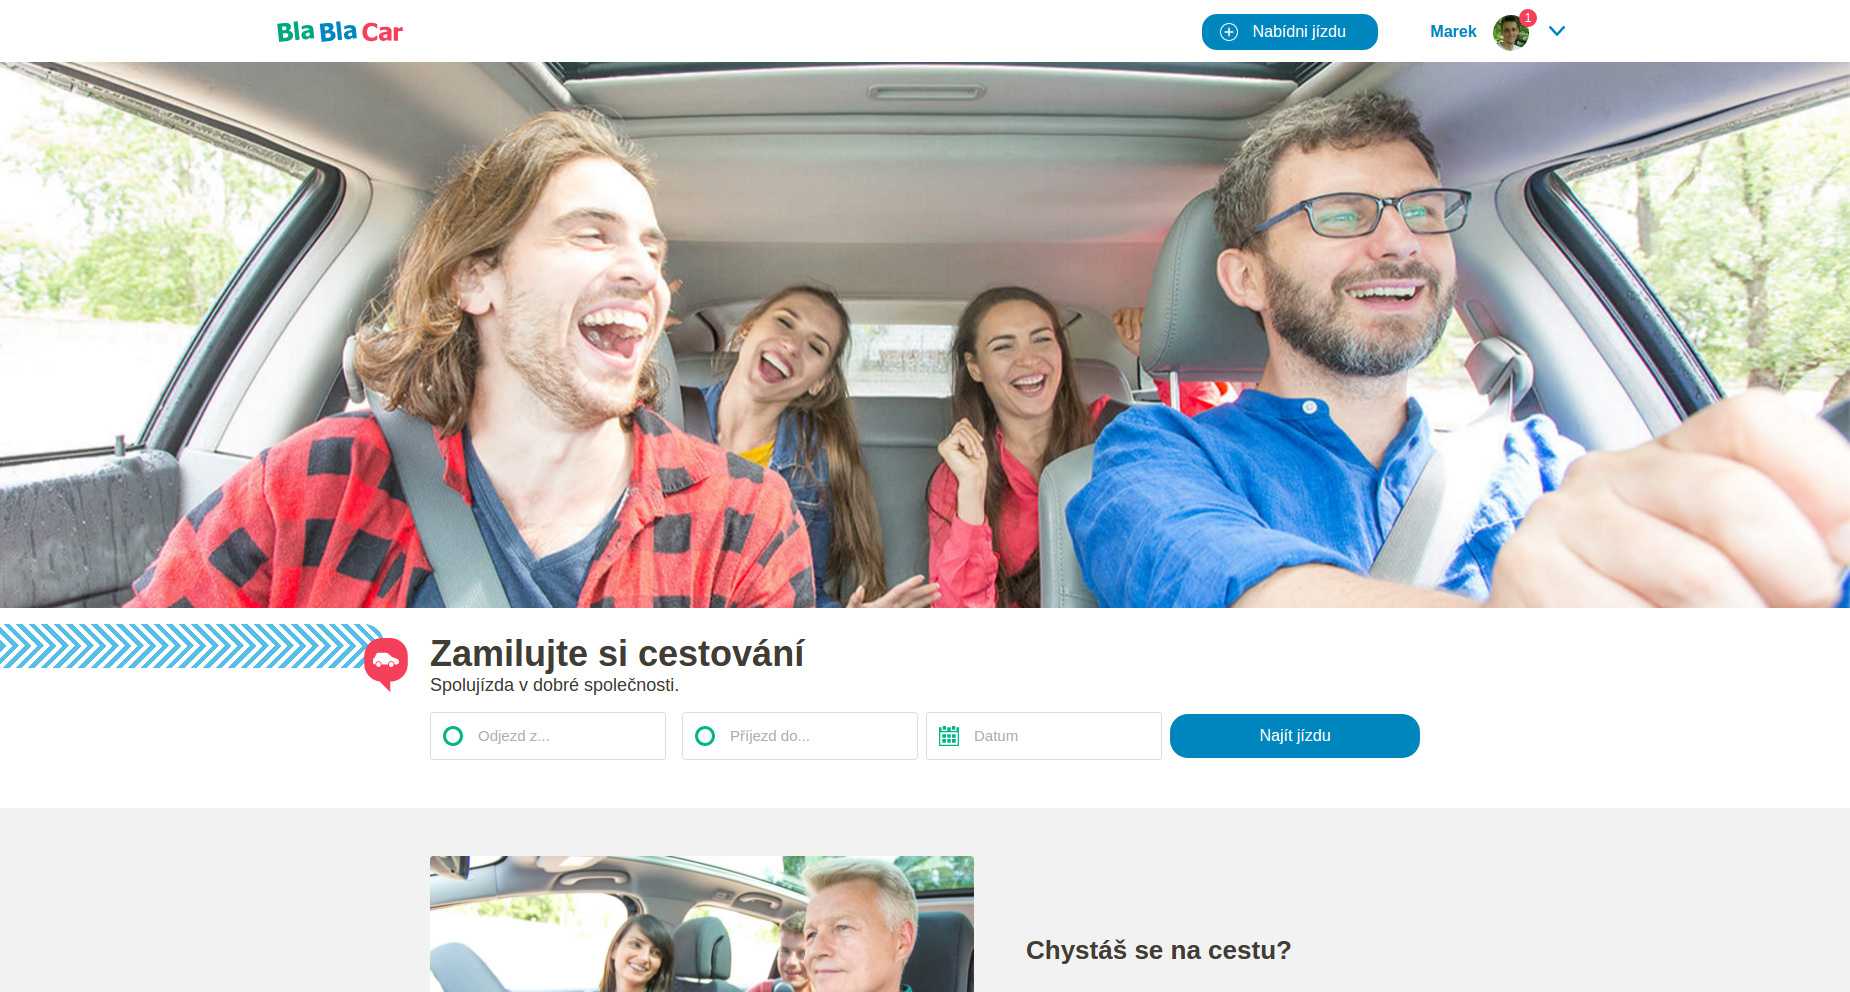
\includegraphics[width=1.0\textwidth]{media/blablacar/homepage.png}
    \caption{BlaBlaCar.cz -- Hlavní stránka}
    \label{fig:blablacar:homepage}
\end{figure}
\subsubsection*{Pozitiva}
\begin{itemize}
    \item[+] \textbf{Přehlednost} -- Na stránce jsou výrazně viditelné dva nejdůležitější typy úkonů a to \textit{Nabídnutí jízdy} a \textit{Vyhledávání jízdy}. I~v~této práci bude brán ohled na to, aby každá důležitá akce měla vysokou prioritu.
    \item[+] \textbf{Ostatní možnosti} -- V~pravém horním rohu je dostupný profil uživatele a nová upozornění na události týkající se uživatelského profilu.
    \item[+] \textbf{Jak to funguje} -- Každému uživateli na první pohled nemusí být jasné, o~co se přesně jedná. Proto web BlaBlaCar.cz na své úvodní stránce uvádí postup jak se na spolujízdu registrovat.
    \item[+] \textbf{Oblíbené trasy} -- Seznam tří nejoblíbenějších tras uživatelů.
\end{itemize}
\subsubsection*{Negativa}
\begin{itemize}
    \item[-] \textbf{Žádná negativa na této stránce nejsou pozorována.}
\end{itemize}


%%%%%%%%%%%%%%%%%%%%%%%%%%%%%%%%%%%%%%%%%%%%%%%%%%%%%%%%%%%%%%%%%%%%%%%%%%%%%%%%%%%%%%%%%%%%%%%%%%%%%%%%%%%%%%%%%%%%%%%%

\newpage
\subsection{Vyhledávání jízdy}
Viz obrázek \ref{fig:blablacar:search}.
\begin{figure}[h]
    \centering
    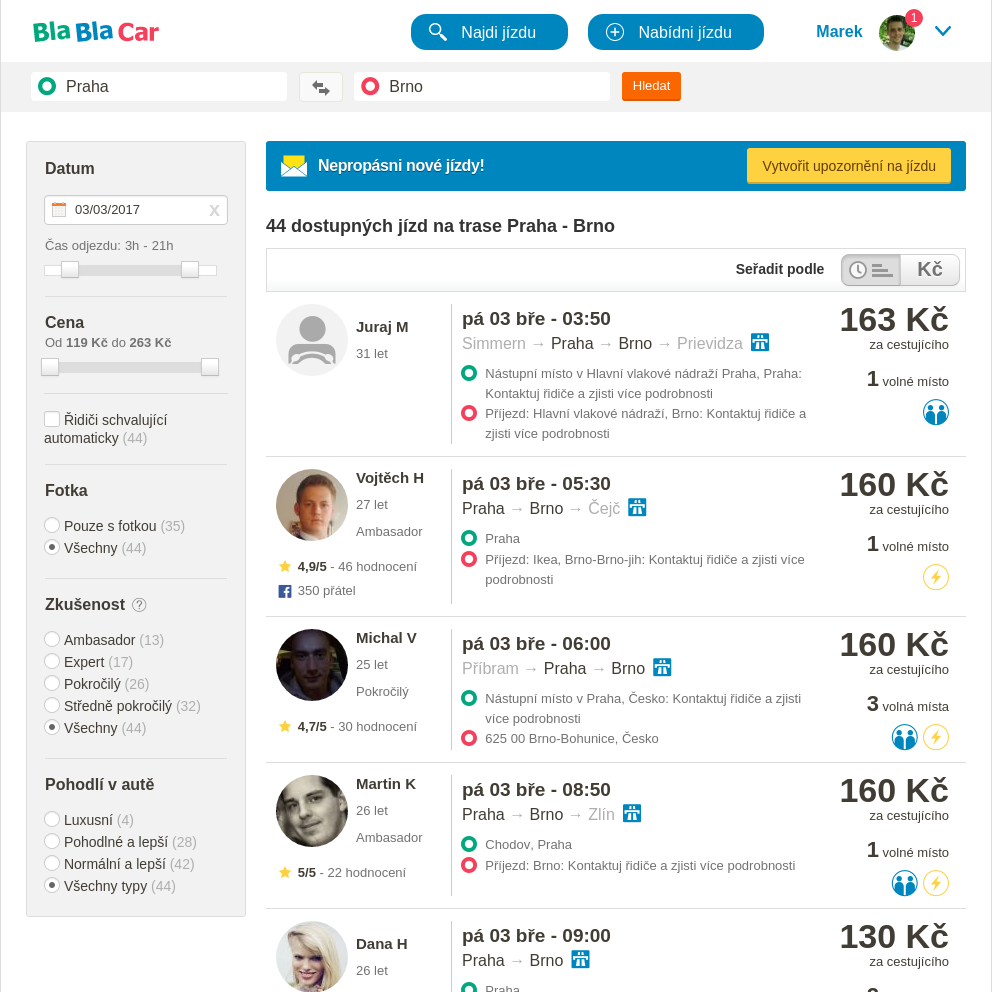
\includegraphics[width=1.0\textwidth]{media/blablacar/search.png}
    \caption{BlaBlaCar.cz -- Vyhledávání nabídek}
    \label{fig:blablacar:search}
\end{figure}
\subsubsection*{Pozitiva}
\begin{itemize}
    \item[+] \textbf{Informativnost} -- Hned na první pohled uživatel vidí všechny relevantní informace: čas, cenu, počet volných míst, délku trasy a hodnocení daného řidiče.
    \item[+] \textbf{Filtry} -- Možnost filtrovaní požadavků na základě zkušeností řidiče a pohodlí auta považuji za nejdůležitější.
    \item[+] \textbf{Možnost řazení} -- Seřazení nabídek podle ceny a času odjezdu je určitě velmi vítaná a potřebná vlastnost.
\end{itemize}
\subsubsection*{Negativa}
\begin{itemize}
    \item[-] \textbf{Nedostupnost profilu řidiče na jeden klik} -- Na první pohled očekávaná funkcionalita (existence předělu mezi cestou a profilem řidiče), při které by se uživatel po kliknutí myší na pravou část nabídky dostal na bližší informace o~jízdě a po kliknutí na levou část nabídky dostal na profil řidiče. Tohoto problému se při návrhu uživatelského rozhraní budu snažit vyvarovat.
\end{itemize}


%%%%%%%%%%%%%%%%%%%%%%%%%%%%%%%%%%%%%%%%%%%%%%%%%%%%%%%%%%%%%%%%%%%%%%%%%%%%%%%%%%%%%%%%%%%%%%%%%%%%%%%%%%%%%%%%%%%%%%%%

\newpage
\subsection{Detail jízdy}
Viz obrázek \ref{fig:blablacar:detail}.
\begin{figure}[h]
    \centering
    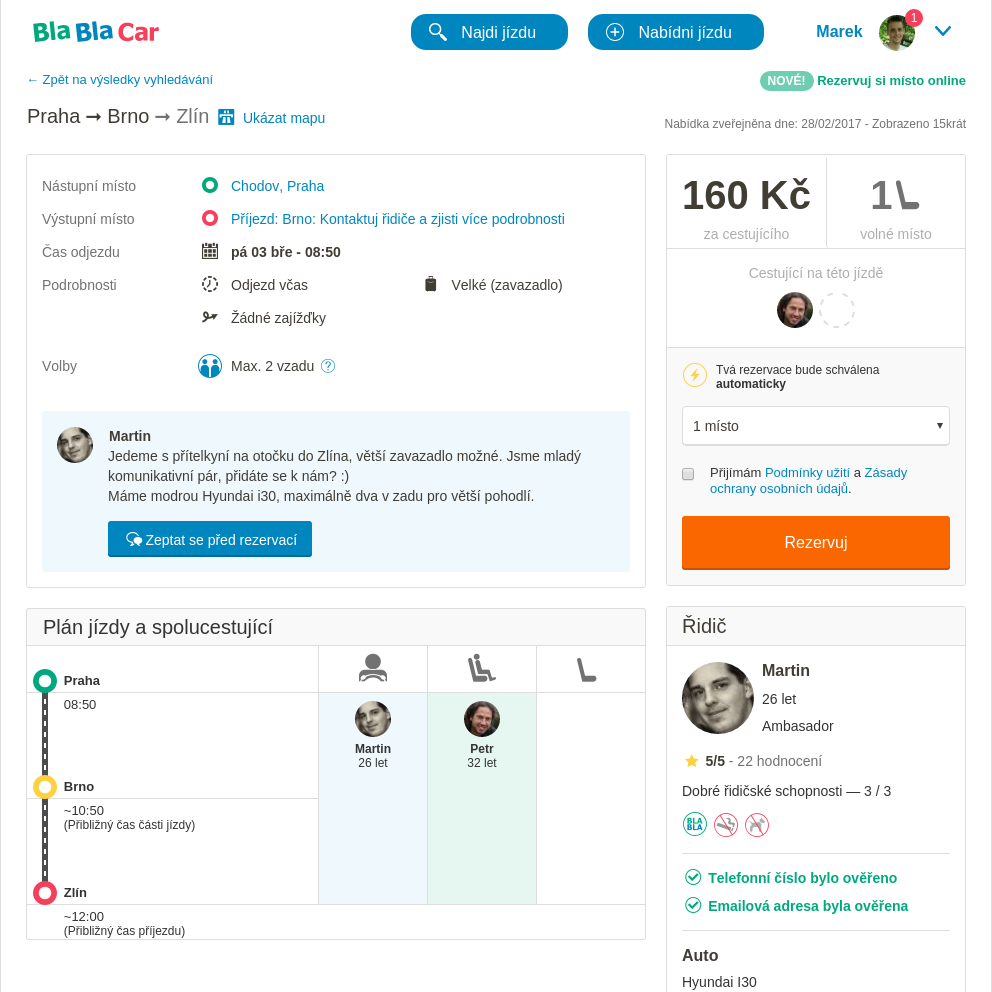
\includegraphics[width=1.0\textwidth]{media/blablacar/detail.png}
    \caption{BlaBlaCar.cz -- Detail jízdy}
    \label{fig:blablacar:detail}
\end{figure}
\subsubsection*{Pozitiva}
\begin{itemize}
    \item[+] \textbf{Harmonogram} -- Graficky velmi pěkně řešený přehled celé jízdy a spolucestujících včetně časů odjezdů a příjezdů.
    \item[+] \textbf{Spolucestující} -- Možnost vidět kdo s~vámi cestuje je vítaná, jelikož s~někým se rádi svezete a někomu se naopak raději vyhnete.
    \item[+] \textbf{Podrobnosti} -- Tímto se řidič vyhne nepříjemnostem s~velkým počtem zavazadel a uživatel s~delšími zajížďkami řidiče.
\end{itemize}
\subsubsection*{Negativa}
\begin{itemize}
    \item[-] \textbf{Žádná negativa na této stránce nejsou pozorována.}
\end{itemize}


%%%%%%%%%%%%%%%%%%%%%%%%%%%%%%%%%%%%%%%%%%%%%%%%%%%%%%%%%%%%%%%%%%%%%%%%%%%%%%%%%%%%%%%%%%%%%%%%%%%%%%%%%%%%%%%%%%%%%%%%

\newpage
\subsection{Nabídnutí jízdy}
Viz obrázky \ref{fig:blablacar:offer} a \ref{fig:blablacar:offer2}.
\begin{figure}[h]
    \centering
    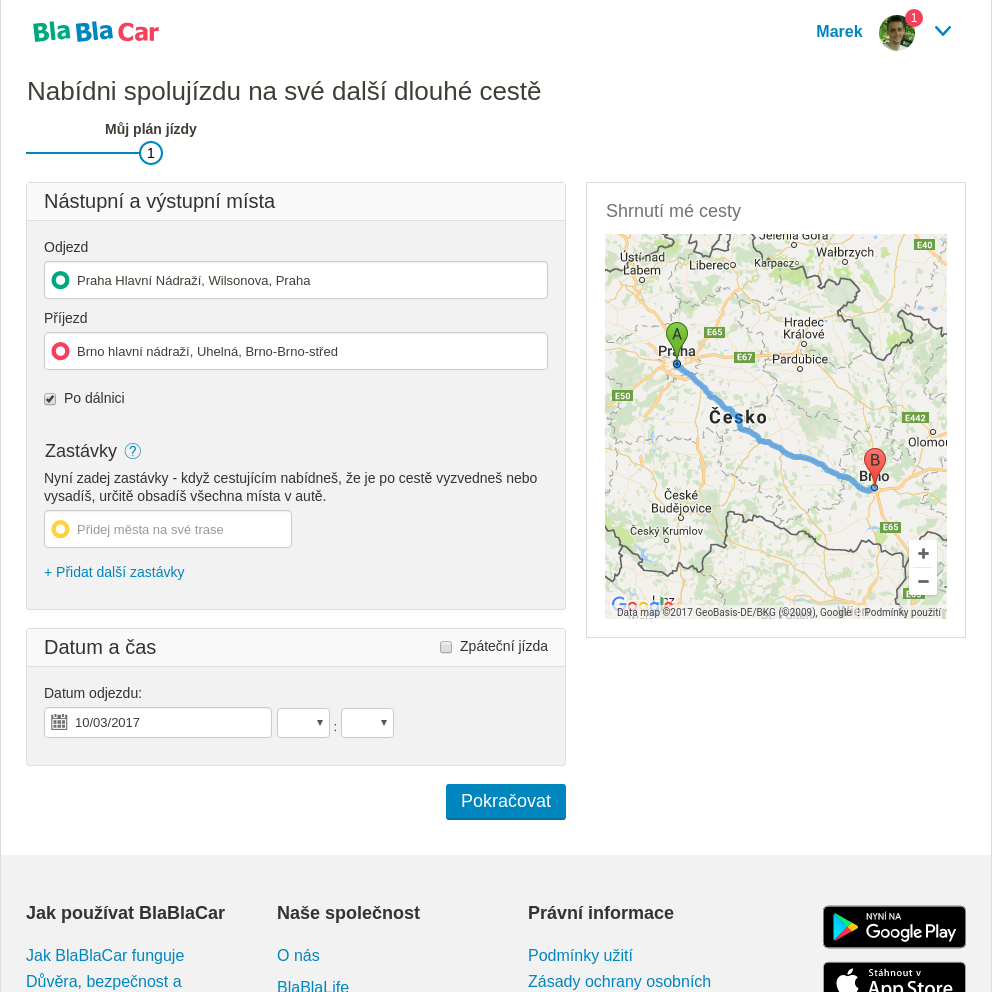
\includegraphics[width=1.0\textwidth]{media/blablacar/offer.png}
    \caption{BlaBlaCar.cz -- Zadání nové jízdy -- Harmonogram}
    \label{fig:blablacar:offer}
\end{figure}
\begin{figure}[h]
    \centering
    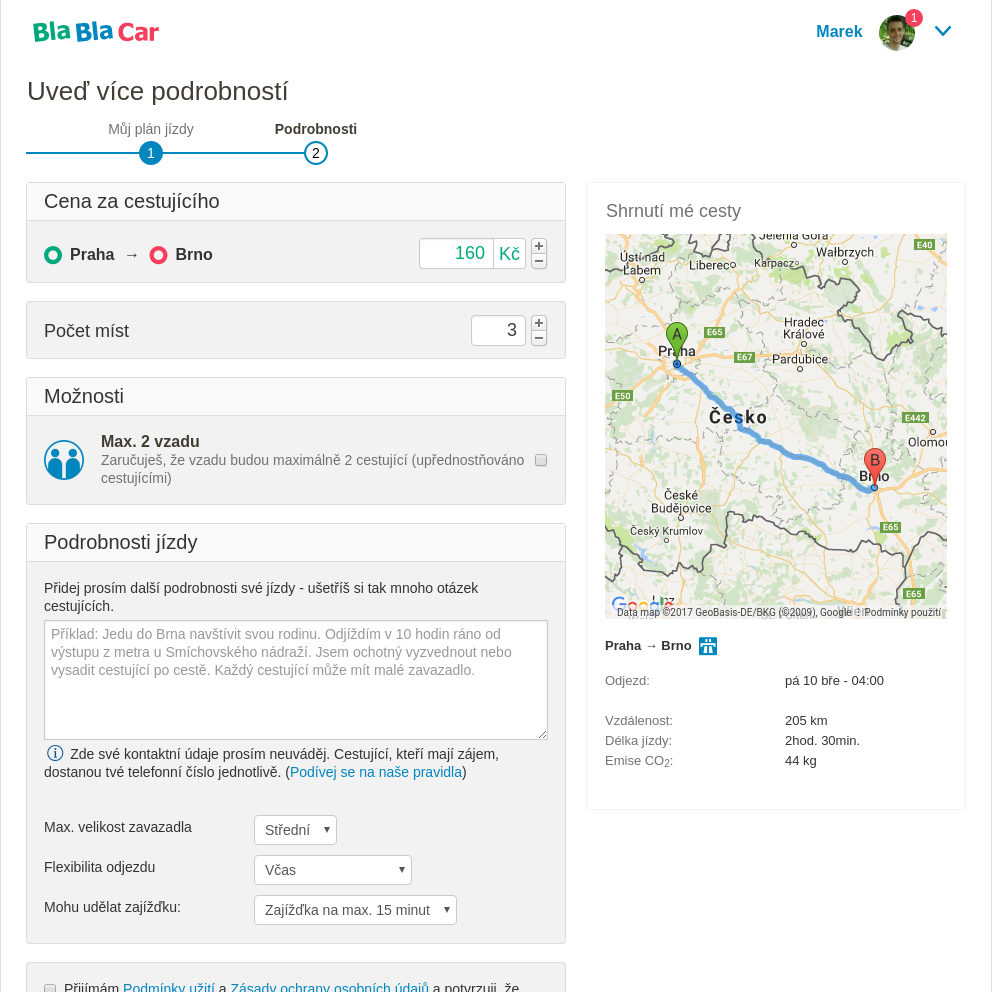
\includegraphics[width=1.0\textwidth]{media/blablacar/offer2.png}
    \caption{BlaBlaCar.cz -- Zadání nové jízdy -- Podrobnosti}
    \label{fig:blablacar:offer2}
\end{figure}
\subsubsection*{Pozitiva}
\begin{itemize}
    \item[+] \textbf{Krok za krokem} -- Uživatel postupně prochází všemi důležitými aspekty nabídky jízdy.
    \item[+] \textbf{Přijatelné UI} -- Všechno je na svém místě a výrazně odlišené od ostatních položek.
    \item[+] \textbf{Doporučená cena} -- Automatické vyplnění ceny na základě ostatních nabídek a vzdálenosti.
    \item[+] \textbf{Mapa} -- Mapa s~celkovým shrnutím vzdálenosti a trvání jízdy.
\end{itemize}
\subsubsection*{Negativa}
\begin{itemize}
    \item[-] \textbf{Žádná negativa na této stránce nejsou pozorována.}
\end{itemize}


%%%%%%%%%%%%%%%%%%%%%%%%%%%%%%%%%%%%%%%%%%%%%%%%%%%%%%%%%%%%%%%%%%%%%%%%%%%%%%%%%%%%%%%%%%%%%%%%%%%%%%%%%%%%%%%%%%%%%%%%

\newpage
\subsection{Profil uživatele}
Viz obrázek \ref{fig:blablacar:profile}.
\begin{figure}[h]
    \centering
    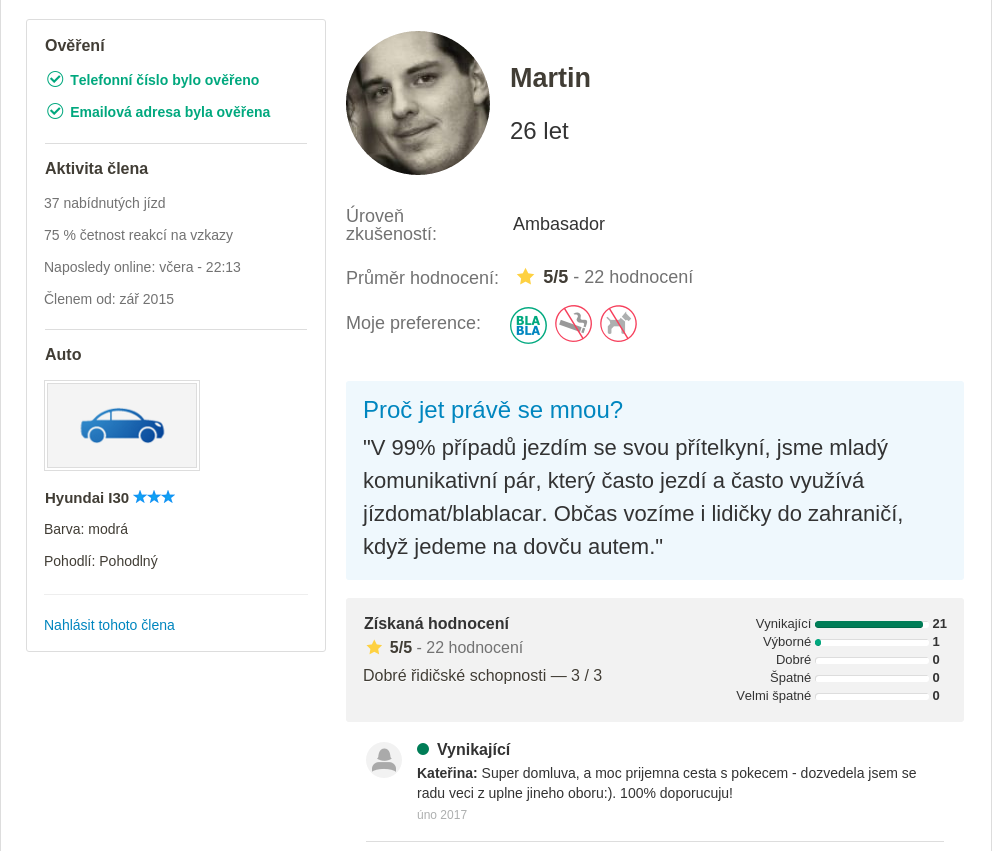
\includegraphics[width=1.0\textwidth]{media/blablacar/profile.png}
    \caption{BlaBlaCar.cz -- Profil uživatele}
    \label{fig:blablacar:profile}
\end{figure}
\subsubsection*{Pozitiva}
\begin{itemize}
    \item[+] \textbf{Informativnost} -- Recenze, typ auta, počet nabídnutých jízd. Uživatel se jednoduše dozví vše, co potřebuje bez nutnosti přecházet na další stránku.
    \item[+] \textbf{Ověření} -- Různé úrovně ověření každého uživatele.
\end{itemize}
\subsubsection*{Negativa}
\begin{itemize}
    \item[-] \textbf{Žádná negativa na této stránce nejsou pozorována.}
\end{itemize}


%%%%%%%%%%%%%%%%%%%%%%%%%%%%%%%%%%%%%%%%%%%%%%%%%%%%%%%%%%%%%%%%%%%%%%%%%%%%%%%%%%%%%%%%%%%%%%%%%%%%%%%%%%%%%%%%%%%%%%%%

\newpage
\subsection{Shrnutí}
Pro účel aplikace jsou nejdůležitější dvě stránky, které BlaBlaCar poskytuje a to \textit{Vyhledávání jízdy} a \textit{Detail jízdy}.

Při návrhu uživatelského rozhraní bude brán zřetel na poskytnutí možnosti filtrování a také seřazení nabídek. Důležité bude zakomponovat rozdílnost kliknutí na uživatele, která uživatele dostane na jeho profil, resp. samotné nabídky, která uživatele přesměruje na bližší informace o~dané nabídce.

I~napříč tomu, že v~aplikaci neexistují spolucestující, tak si beru příklad z~této vlastnosti BlaBlaCar a v~detailu nabídky zvážím výpis historie s~daným uživatelem, která slouží velmi podobnému účelu.

Hodnocení uživatelů je řešeno pomocí až pěti hvězdiček.